\sourcepageanchor{298}
\subsection{评价估计量的方法}\label{sec:7.3}
上一节介绍了构造参数点估计量的一些合理技巧.不过，一个困难随之出现：在具体情形中通常不止一种方法可用，因此经常需要在不同估计量之间作选择.当然，不同构造方法可能给出相同答案，使评价稍微容易些；但很多时候，不同方法会产生不同估计量.

评价统计程序的一般问题，属于称为决策论（decision theory）的统计学分支，\autoref{sec:7.3.4}将较详细地介绍它.不过，在获得一些关于性能的线索之前，不应考虑采用任何程序.本节将介绍评价估计量的若干基本准则，并据此考察一些估计量.
\subsubsection{均方误差}\label{sec:7.3.1}
先研究在有限样本下衡量估计量质量的方法，从均方误差开始.
\begin{definition}\label{def:7.3.1}\index{SI0683@均方误差}
参数$\theta$的估计量$W$的均方误差（mean squared error，MSE）是定义为$E_\theta(W-\theta)^2$的$\theta$的函数.
\end{definition}
注意，MSE衡量估计量$W$与参数$\theta$之差的平方的平均值，作为点估计量的性能指标是相当合理的.一般而言，绝对距离$|W-\theta|$的任意递增函数都可用来衡量估计量的好坏（平均绝对误差$E_\theta(|W-\theta|)$是一个合理替代）.但MSE比其他距离指标至少有两个优点：首先，解析处理十分方便；其次，它具有如下解释：
\begin{equation}\label{eq:7.3.1}\index{SI0801@方差}
E_\theta(W-\theta)^2=\operatorname{Var}_\theta W+(E_\theta W-\theta)^2=\operatorname{Var}_\theta W+(\operatorname{Bias}_\theta W)^2,
\end{equation}
其中，估计量的偏差定义如下.
\begin{definition}\label{def:7.3.2}\index{SI0090@偏差}\index{SI1044@无偏估计量}
参数$\theta$的点估计量$W$的偏差（bias），是$W$的期望与$\theta$之差，即$\operatorname{Bias}_\theta W=E_\theta W-\theta$.偏差作为$\theta$的函数恒等于零的估计量，称为无偏估计量（unbiased estimator），它对所有$\theta$满足$E_\theta W=\theta$.
\end{definition}
因此，MSE包括两个分量：一个衡量估计量的变异性（精密度，precision），另一个衡量其偏差（准确度，accuracy）.具有良好MSE性质的估计量，其方差与偏差的组合较小.为了找到MSE性质良好的估计量，需要寻找同时控制方差和偏差的估计量.显然，无偏估计量在控制偏差方面做得很好.

对于无偏估计量，有
$$E_\theta(W-\theta)^2=\operatorname{Var}_\theta W,$$
所以，估计量若无偏，其MSE就等于方差.
\begin{example}[正态分布的MSE]\label{ex:7.3.3}\index{SI1055@正态}
设$X_1,\ldots,X_n$独立同分布于$n(\mu,\sigma^2)$.统计量$\bar X$与$S^2$都是无偏估计量，因为
$$E\bar X=\mu,\qquad ES^2=\sigma^2,\qquad\text{对所有 }\mu\text{ 和 }\sigma^2.$$
\sourcepageanchor{299}
（不假设正态性时也成立，见\autoref{thm:5.2.6}.）这些估计量的MSE为
\begin{align*}
E(\bar X-\mu)^2&=\operatorname{Var}\bar X=\frac{\sigma^2}n,\\
E(S^2-\sigma^2)^2&=\operatorname{Var}S^2=\frac{2\sigma^4}{n-1}.
\end{align*}
即使去掉正态性假设，$\bar X$的MSE仍为$\sigma^2/n$.不过，若放宽正态性假设，上面$S^2$的MSE表达式便不再相同（见\autoref{exercise:5.8}）.
\end{example}
虽然从MSE角度看，很多无偏估计量也很合理，但应注意，控制偏差并不保证控制MSE.特别地，有时方差与偏差之间存在权衡：以较小的偏差增加换取较大的方差减少，从而改善MSE.
\begin{example}[续\autoref{ex:7.3.3}]\label{ex:7.3.4}
$\sigma^2$的另一个估计量是极大似然估计量$\widehat\sigma^2=\frac1n\sum_{i=1}^n(X_i-\bar X)^2=\frac{n-1}nS^2$.直接计算得
$$E\widehat\sigma^2=E\left(\frac{n-1}nS^2\right)=\frac{n-1}n\sigma^2,$$
所以$\widehat\sigma^2$是$\sigma^2$的有偏估计量.其方差也可算出：
$$\operatorname{Var}\widehat\sigma^2=\operatorname{Var}\left(\frac{n-1}nS^2\right)=\left(\frac{n-1}n\right)^2\operatorname{Var}S^2=\frac{2(n-1)\sigma^4}{n^2},$$
因此，MSE为
$$E(\widehat\sigma^2-\sigma^2)^2=\frac{2(n-1)\sigma^4}{n^2}+\left(\frac{n-1}n\sigma^2-\sigma^2\right)^2=\left(\frac{2n-1}{n^2}\right)\sigma^4.$$
于是有
$$E(\widehat\sigma^2-\sigma^2)^2=\left(\frac{2n-1}{n^2}\right)\sigma^4<\left(\frac2{n-1}\right)\sigma^4=E(S^2-\sigma^2)^2,$$
表明$\widehat\sigma^2$的MSE小于$S^2$.因此，通过以偏差换取方差的减少，MSE得到改善.
\end{example}
必须立即指出，上例并不意味着应放弃用$S^2$估计$\sigma^2$.上述论证表明，如果用MSE衡量，平均而言$\widehat\sigma^2$比$S^2$更接近$\sigma^2$.不过，$\widehat\sigma^2$有偏，而且平均而言会低估$\sigma^2$.仅此一点就可能使我们对用$\widehat\sigma^2$估计$\sigma^2$感到不安.此外，也可以认为，MSE虽是位置参数的合理准则，却不是尺度参数的合理准则，因此根本不应作上述比较.（问题之一是，MSE对高估与低估施加同等惩罚，在位置参数情形中这没有问题.但对尺度参数，零是一个自然下界，所以估计问题并不对称.此时用MSE往往对低估较为宽容.）最终结果并不是获得绝对的答案，而是收集更多关于估计量的信息，希望对具体情形选择一个好的估计量.
\sourcepageanchor{300}
一般而言，由于MSE是参数的函数，并不存在一个“最佳”估计量.两个估计量的MSE曲线往往相交，说明每个估计量只在参数空间的一部分中优于另一个.不过，即使这种局部信息，有时也能指导我们在估计量之间作选择.
\begin{example}[二项Bayes估计量的MSE]\label{ex:7.3.5}\index{SI0079@伯努利}\index{SI0800@伯努利}
设$X_1,\ldots,X_n$独立同分布于$\operatorname{Bernoulli}(p)$.$\bar X$作为$p$的估计量，其MSE为
$$E_p(\bar X-p)^2=\operatorname{Var}_p\bar X=\frac{p(1-p)}n.$$
令$Y=\sum X_i$，回顾\autoref{ex:7.2.14}中得到的Bayes估计量$\widehat p_B=(Y+\alpha)/(\alpha+\beta+n)$.它作为$p$的估计量，其MSE为
\begin{align*}
E_p(\widehat p_B-p)^2&=\operatorname{Var}_p\widehat p_B+(\operatorname{Bias}_p\widehat p_B)^2\\
&=\operatorname{Var}_p\left(\frac{Y+\alpha}{\alpha+\beta+n}\right)+\left(E_p\left(\frac{Y+\alpha}{\alpha+\beta+n}\right)-p\right)^2\\
&=\frac{np(1-p)}{(\alpha+\beta+n)^2}+\left(\frac{np+\alpha}{\alpha+\beta+n}-p\right)^2.
\end{align*}
在没有关于$p$的良好先验信息时，可以尝试选择$\alpha$和$\beta$，使$\widehat p_B$的MSE为常数.细节不难算出（见\autoref{exercise:7.33}），取$\alpha=\beta=\sqrt{n/4}$便得到
$$\widehat p_B=\frac{Y+\sqrt{n/4}}{n+\sqrt n}\qquad\text{且}\qquad E(\widehat p_B-p)^2=\frac n{4(n+\sqrt n)^2}.$$
\begin{figure}[H]
\centering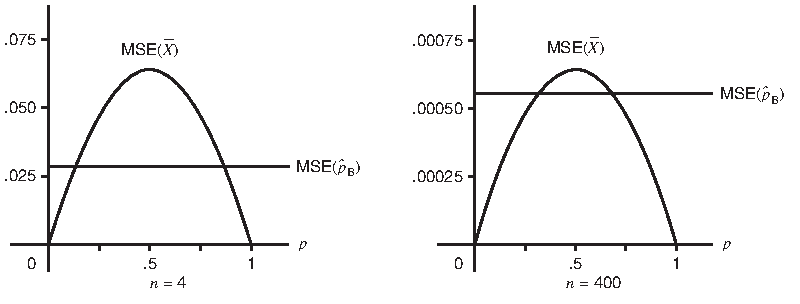
\includegraphics[width=.95\linewidth]{assets/chapter7/fig-7-3-1.pdf}
\caption{\autoref{ex:7.3.5}中，样本量$n=4$与$n=400$时$\bar X$和$\widehat p_B$的MSE比较}\label{fig:7.3.1}
\end{figure}
若想根据MSE在$\widehat p_B$与$\bar X$之间选择，\autoref{fig:7.3.1}很有帮助.$n$较小时，$\widehat p_B$是更好的选择（除非坚信$p$接近0或1）；$n$较大时，$\bar X$是更好的选择（除非坚信$p$接近$1/2$）.虽然MSE准则没有说明一个估计量一致优于另一个，但仍提供了有用信息.将这些信息与对实际问题的了解结合起来，就能为具体情形选出较好的估计量.
\end{example}
\sourcepageanchor{301}
在某些情形中，尤其估计位置参数时，MSE有助于在一类等变估计量中寻找最佳者（\autoref{sec:6.4}）.对群$\mathcal G$中固定的$g$，用$\bar g(\theta)$表示把$\theta$映到$\theta'$的函数，即$\bar g(\theta)=\theta'$.若$W(\boldsymbol X)$估计$\theta$，则有
\begin{quote}
测量等变性：$W(\boldsymbol x)$估计$\theta$ $\Rightarrow$ $\bar g(W(\boldsymbol x))$估计$\bar g(\theta)=\theta'$.

形式不变性：\index{SI0788@形式化}\semanticindexanchor{788:301}$W(\boldsymbol x)$估计$\theta$ $\Rightarrow$ $W(g(\boldsymbol x))$估计$\bar g(\theta)=\theta'$.
\end{quote}
将这两个要求结合，得到$W(g(\boldsymbol x))=\bar g(W(\boldsymbol x))$.
\begin{example}[等变估计量的MSE]\label{ex:7.3.6}\index{SI0464@位置}\index{SI0789@均方误差}
设$X_1,\ldots,X_n$独立同分布于$f(x-\theta)$.估计量$W(X_1,\ldots,X_n)$若满足$W(g_a(\boldsymbol x))=\bar g_a(W(\boldsymbol x))$，就必须有
\begin{equation}\label{eq:7.3.2}
W(x_1,\ldots,x_n)+a=W(x_1+a,\ldots,x_n+a),
\end{equation}
它规定了关于变换群$\mathcal G=\{g_a(\boldsymbol x):-\infty<a<\infty\}$的等变估计量，其中$g_a(x_1,\ldots,x_n)=(x_1+a,\ldots,x_n+a)$.对这些估计量，有
\begin{equation}\label{eq:7.3.3}
\begin{aligned}
&E_\theta(W(X_1,\ldots,X_n)-\theta)^2\\
&=E_\theta(W(X_1+a,\ldots,X_n+a)-a-\theta)^2\\
&=E_\theta(W(X_1-\theta,\ldots,X_n-\theta))^2\qquad(a=-\theta)\\
&=\int_{-\infty}^\infty\cdots\int_{-\infty}^\infty(W(x_1-\theta,\ldots,x_n-\theta))^2\prod_{i=1}^nf(x_i-\theta)\,dx_i\\
&=\int_{-\infty}^\infty\cdots\int_{-\infty}^\infty(W(u_1,\ldots,u_n))^2\prod_{i=1}^nf(u_i)\,du_i.\quad(u_i=x_i-\theta)
\end{aligned}
\end{equation}
最后一个表达式不依赖$\theta$，所以这些等变估计量的MSE不是$\theta$的函数.因而可以用MSE排列它们的优劣，并找到MSE最小的等变估计量.实际上，这一估计量是如下数学问题的解：在约束\eqref{eq:7.3.2}下，寻找使\eqref{eq:7.3.3}最小的函数$W$.（见\autoref{exercise:7.35}和\autoref{exercise:7.36}.）
\end{example}
\subsubsection{最佳无偏估计量}\label{sec:7.3.2}
如上一小节所述，基于MSE比较估计量，未必能选出明确的优胜者.事实上，不存在一个“最佳MSE”估计量.很多人觉得这令人烦恼，希望得到一个“推荐”的估计量，而不愿逐一比较候选者的MSE.

不存在一个“最佳MSE”估计量，是因为所有估计量构成的类太大.（例如，在$\theta=17$处，估计量$\widehat\theta=17$的MSE无可超越，但在其他地方它是一个很差的估计量.）使寻找“最佳”估计量的问题变得可处理的一种办法，是限制估计量的类.一种常用限制方式，也是本小节要考虑的方式，就是只考虑无偏估计量.

若$W_1$和$W_2$都是参数$\theta$的无偏估计量，即$E_\theta W_1=E_\theta W_2=\theta$，那么它们的均方误差等于方差，因此应选择方差较小的估计量.若能找到方差一致最小的无偏估计量——最佳无偏估计量——任务便完成了.

继续之前要指出，虽然我们将讨论无偏估计量，但本小节及下一小节的结果实际上更一般.设$W^*$是$\theta$的一个估计量，满足$E_\theta W^*=\tau(\theta)\ne\theta$，而我们希望考察$W^*$的价值.考虑估计量类
$$\mathcal C_\tau=\{W:E_\theta W=\tau(\theta)\}.$$
\sourcepageanchor{302}
对任意$W_1,W_2\in\mathcal C_\tau$，有$\operatorname{Bias}_\theta W_1=\operatorname{Bias}_\theta W_2$，所以
$$E_\theta(W_1-\theta)^2-E_\theta(W_2-\theta)^2=\operatorname{Var}_\theta W_1-\operatorname{Var}_\theta W_2,$$
在$\mathcal C_\tau$内部作MSE比较，只需比较方差.因此，虽然使用无偏估计量的措辞，我们实际比较的是具有相同期望$\tau(\theta)$的估计量.

本小节的目标是研究寻找“最佳”无偏估计量的方法，其定义如下.
\begin{definition}\label{def:7.3.7}\index{SI1045@最优}
若估计量$W^*$对所有$\theta$满足$E_\theta W^*=\tau(\theta)$，而且对于任一其他满足$E_\theta W=\tau(\theta)$的估计量$W$，对所有$\theta$都有$\operatorname{Var}_\theta W^*\le\operatorname{Var}_\theta W$，则$W^*$称为$\tau(\theta)$的最佳无偏估计量（best unbiased estimator）.$W^*$也称为$\tau(\theta)$的一致最小方差无偏估计量（uniform minimum variance unbiased estimator，UMVUE）.
\end{definition}
由于许多原因，寻找最佳无偏估计量（假如存在的话！）并不容易.下例展示其中两个原因.
\begin{example}[Poisson分布的无偏估计]\label{ex:7.3.8}\index{SI1057@泊松}
设$X_1,\ldots,X_n$独立同分布于$\operatorname{Poisson}(\lambda)$，$\bar X$和$S^2$分别为样本均值与样本方差.回顾Poisson分布的均值和方差均等于$\lambda$.因此，应用\autoref{thm:5.2.6}得到
$$E_\lambda\bar X=\lambda,\qquad\text{对所有 }\lambda,$$
以及
$$E_\lambda S^2=\lambda,\qquad\text{对所有 }\lambda,$$
所以$\bar X$与$S^2$都是$\lambda$的无偏估计量.

为了确定$\bar X$与$S^2$中哪个更好，应比较方差.同样由\autoref{thm:5.2.6}，有$\operatorname{Var}_\lambda\bar X=\lambda/n$，但$\operatorname{Var}_\lambda S^2$的计算很长（类似\hyperref[exercise:5.10]{习题5.10(b)}）.这是寻找最佳无偏估计量首先遇到的问题之一：计算不仅冗长繁琐，还可能白费力气（本例即如此），因为我们将看到，对所有$\lambda$都有$\operatorname{Var}_\lambda\bar X\le\operatorname{Var}_\lambda S^2$.

即使能够确立$\bar X$优于$S^2$，还要考虑估计量类
$$W_a(\bar X,S^2)=a\bar X+(1-a)S^2.$$
对任意常数$a$，都有$E_\lambda W_a(\bar X,S^2)=\lambda$，所以现在有无穷多个$\lambda$的无偏估计量.即使$\bar X$优于$S^2$，它也优于每个$W_a(\bar X,S^2)$吗？而且，如何确信没有其他更好的无偏估计量隐藏在别处？
\end{example}
这个例子展示了寻找最佳无偏估计量时可能遇到的若干问题，也提示需要一种更全面的方法.假设要估计分布$f(\boldsymbol x\mid\theta)$的参数$\tau(\theta)$，能够给出任一无偏估计量方差的下界，记为$B(\theta)$.若能找到无偏估计量$W^*$满足$\operatorname{Var}_\theta W^*=B(\theta)$，便找到了最佳无偏估计量.这就是使用Cramér--Rao下界（Cramér--Rao lower bound）的思路.
\begin{theorem}[Cramér--Rao不等式]\label{thm:7.3.9}\index{SI0228@Cramér–Rao下界}
设$X_1,\ldots,X_n$是具有pdf $f(\boldsymbol x\mid\theta)$的样本，$W(\boldsymbol X)=W(X_1,\ldots,X_n)$为满足下列条件的任意估计量：
\begin{equation}\label{eq:7.3.4}
\begin{aligned}
\frac d{d\theta}E_\theta W(\boldsymbol X)&=\int_{\mathcal X}\frac\partial{\partial\theta}[W(\boldsymbol x)f(\boldsymbol x\mid\theta)]\,d\boldsymbol x,\\
\text{且}\qquad\operatorname{Var}_\theta W(\boldsymbol X)&<\infty.
\end{aligned}
\end{equation}
\sourcepageanchor{303}
则
\begin{equation}\label{eq:7.3.5}
\operatorname{Var}_\theta(W(\boldsymbol X))\ge\frac{\bigl(\frac d{d\theta}E_\theta W(\boldsymbol X)\bigr)^2}{E_\theta\left(\left(\frac\partial{\partial\theta}\log f(\boldsymbol X\mid\theta)\right)^2\right)}.
\end{equation}
\end{theorem}
\begin{proof}
此定理的证明简洁优美，是对Cauchy--Schwarz不等式的巧妙应用；用统计语言说，就是对任意两个随机变量$X$和$Y$都有
\begin{equation}\label{eq:7.3.6}
[\operatorname{Cov}(X,Y)]^2\le(\operatorname{Var}X)(\operatorname{Var}Y).
\end{equation}
重新整理\eqref{eq:7.3.6}，可得$X$的方差下界：
$$\operatorname{Var}X\ge\frac{[\operatorname{Cov}(X,Y)]^2}{\operatorname{Var}Y}.$$
这个定理的巧妙之处，在于选$X$为估计量$W(\boldsymbol X)$，选$Y$为$\frac\partial{\partial\theta}\log f(\boldsymbol X\mid\theta)$，然后应用Cauchy--Schwarz不等式.

首先注意
\begin{equation}\label{eq:7.3.7}
\begin{aligned}
\frac d{d\theta}E_\theta W(\boldsymbol X)&=\int_{\mathcal X}W(\boldsymbol x)\left[\frac\partial{\partial\theta}f(\boldsymbol x\mid\theta)\right]d\boldsymbol x\\
&=E_\theta\left[W(\boldsymbol X)\frac{\frac\partial{\partial\theta}f(\boldsymbol X\mid\theta)}{f(\boldsymbol X\mid\theta)}\right]\quad\text{（乘以$f/f$）}\\
&=E_\theta\left[W(\boldsymbol X)\frac\partial{\partial\theta}\log f(\boldsymbol X\mid\theta)\right],\quad\text{（对数的性质）}
\end{aligned}
\end{equation}
这提示了$W(\boldsymbol X)$与$\frac\partial{\partial\theta}\log f(\boldsymbol X\mid\theta)$之间的协方差.要成为协方差，还须减去期望的乘积，因此计算$E_\theta(\frac\partial{\partial\theta}\log f(\boldsymbol X\mid\theta))$.若取$W(\boldsymbol x)=1$应用\eqref{eq:7.3.7}，有\footnote{译注：这一步还要求微分与积分的交换对$W\equiv1$成立，而定理原述仅对所考察的$W$列出\eqref{eq:7.3.4}.通常的正则性条件还保证此项交换、共同支撑以及所用信息量为正且有限；应用定理时须一并检查，不能仅凭某个$W$的交换条件推出得分期望为零.}
\begin{equation}\label{eq:7.3.8}
E_\theta\left(\frac\partial{\partial\theta}\log f(\boldsymbol X\mid\theta)\right)=\frac d{d\theta}E_\theta[1]=0.
\end{equation}
因此，$\operatorname{Cov}_\theta(W(\boldsymbol X),\frac\partial{\partial\theta}\log f(\boldsymbol X\mid\theta))$等于乘积的期望，由\eqref{eq:7.3.7}和\eqref{eq:7.3.8}可得
\begin{equation}\label{eq:7.3.9}
\begin{aligned}
\operatorname{Cov}_\theta\left(W(\boldsymbol X),\frac\partial{\partial\theta}\log f(\boldsymbol X\mid\theta)\right)
&=E_\theta\left(W(\boldsymbol X)\frac\partial{\partial\theta}\log f(\boldsymbol X\mid\theta)\right)\\
&=\frac d{d\theta}E_\theta W(\boldsymbol X).
\end{aligned}
\end{equation}
另外，由于$E_\theta(\frac\partial{\partial\theta}\log f(\boldsymbol X\mid\theta))=0$，有
\begin{equation}\label{eq:7.3.10}
\operatorname{Var}_\theta\left(\frac\partial{\partial\theta}\log f(\boldsymbol X\mid\theta)\right)=E_\theta\left(\left(\frac\partial{\partial\theta}\log f(\boldsymbol X\mid\theta)\right)^2\right).
\end{equation}
结合Cauchy--Schwarz不等式、\eqref{eq:7.3.9}和\eqref{eq:7.3.10}，得到
$$\operatorname{Var}_\theta(W(\boldsymbol X))\ge\frac{\bigl(\frac d{d\theta}E_\theta W(\boldsymbol X)\bigr)^2}{E_\theta\left(\left(\frac\partial{\partial\theta}\log f(\boldsymbol X\mid\theta)\right)^2\right)},$$
定理得证.
\end{proof}
\sourcepageanchor{304}
若再加上样本独立的假设，下界的计算便得到简化.分母中的期望化为一元计算，如下述推论所示.
\begin{corollary}[Cramér--Rao不等式，独立同分布情形]\label{cor:7.3.10}
若\autoref{thm:7.3.9}的假设满足，而且$X_1,\ldots,X_n$独立同分布，具有pdf $f(x\mid\theta)$，则
$$\operatorname{Var}_\theta W(\boldsymbol X)\ge\frac{\bigl(\frac d{d\theta}E_\theta W(\boldsymbol X)\bigr)^2}{nE_\theta\left(\left(\frac\partial{\partial\theta}\log f(X\mid\theta)\right)^2\right)}.$$
\end{corollary}
\begin{proof}
只需证明
$$E_\theta\left(\left(\frac\partial{\partial\theta}\log f(\boldsymbol X\mid\theta)\right)^2\right)=nE_\theta\left(\left(\frac\partial{\partial\theta}\log f(X\mid\theta)\right)^2\right).$$
由于$X_1,\ldots,X_n$相互独立，
\begin{equation}\label{eq:7.3.11}
\begin{aligned}
E_\theta\left(\frac\partial{\partial\theta}\log f(\boldsymbol X\mid\theta)\right)^2
&=E_\theta\left(\left(\frac\partial{\partial\theta}\log\prod_{i=1}^nf(X_i\mid\theta)\right)^2\right)\\
&=E_\theta\left(\left(\sum_{i=1}^n\frac\partial{\partial\theta}\log f(X_i\mid\theta)\right)^2\right)\quad\text{（对数性质）}\\
&=\sum_{i=1}^nE_\theta\left(\left(\frac\partial{\partial\theta}\log f(X_i\mid\theta)\right)^2\right)\quad\text{（展开平方）}\\
&\quad+\sum_{i\ne j}E_\theta\left(\frac\partial{\partial\theta}\log f(X_i\mid\theta)\frac\partial{\partial\theta}\log f(X_j\mid\theta)\right).
\end{aligned}
\end{equation}
对于$i\ne j$，有
\begin{align*}
&E_\theta\left(\frac\partial{\partial\theta}\log f(X_i\mid\theta)\frac\partial{\partial\theta}\log f(X_j\mid\theta)\right)\\
&\quad=E_\theta\left(\frac\partial{\partial\theta}\log f(X_i\mid\theta)\right)E_\theta\left(\frac\partial{\partial\theta}\log f(X_j\mid\theta)\right)\quad\text{（独立性）}\\
&\quad=0.\qquad\text{（由\eqref{eq:7.3.8}）}
\end{align*}
所以\eqref{eq:7.3.11}的第二个和为零，第一个和为
\begin{align*}
&\sum_{i=1}^nE_\theta\left(\left(\frac\partial{\partial\theta}\log f(X_i\mid\theta)\right)^2\right)\\
&\qquad=nE_\theta\left(\left(\frac\partial{\partial\theta}\log f(X\mid\theta)\right)^2\right),\qquad\text{（同分布）}
\end{align*}
从而确立推论.
\end{proof}
继续之前指出，虽然Cramér--Rao下界是针对连续随机变量陈述的，但它也适用于离散随机变量.允许交换积分与微分的关键条件\eqref{eq:7.3.4}，只需作显然的修改.若$f(x\mid\theta)$是pmf，就必须能够交换微分与求和.（当然，这假设虽然$f(x\mid\theta)$是pmf，关于$x$不可微，但关于$\theta$可微.大多数常见pmf都如此.）
\sourcepageanchor{305}
量$E_\theta((\frac\partial{\partial\theta}\log f(\boldsymbol X\mid\theta))^2)$称为样本的信息数（information number），或Fisher信息（Fisher information）.\index{SI0582@信息量}\semanticindexanchor{582:305}这个术语反映了如下事实：信息数给出了$\theta$的最佳无偏估计量方差的下界.信息数越大，即关于$\theta$的信息越多，最佳无偏估计量的方差下界就越小.

事实上，Cramér--Rao不等式也称信息不等式（Information Inequality），而信息不等式存在比这里更一般的形式.更一般形式的一个关键区别，是去掉对候选估计量的全部假设，改为对潜在密度作假设.在这种形式下，信息不等式对于比较估计量性能十分有用.细节见\hyperref[bib:source200]{Lehmann和Casella（1998）}第2.6节.

现在，对于任意可微函数$\tau(\theta)$，我们得到了满足\eqref{eq:7.3.4}及$E_\theta W=\tau(\theta)$的任意估计量$W$的方差下界.此下界只依赖于$\tau(\theta)$和$f(\boldsymbol x\mid\theta)$，是方差的一致下界.任何满足$E_\theta W=\tau(\theta)$且达到下界的候选估计量，都是$\tau(\theta)$的最佳无偏估计量.

在看例子之前，先给出一个有助于应用此定理的计算结果.证明留作\autoref{exercise:7.39}.
\begin{lemma}\label{lem:7.3.11}
若$f(x\mid\theta)$满足
$$\frac d{d\theta}E_\theta\left(\frac\partial{\partial\theta}\log f(X\mid\theta)\right)=\int\frac\partial{\partial\theta}\left[\left(\frac\partial{\partial\theta}\log f(x\mid\theta)\right)f(x\mid\theta)\right]dx$$
（指数族满足此条件），则
$$E_\theta\left(\left(\frac\partial{\partial\theta}\log f(X\mid\theta)\right)^2\right)=-E_\theta\left(\frac{\partial^2}{\partial\theta^2}\log f(X\mid\theta)\right).$$
\end{lemma}
利用刚建立的工具，回到Poisson例子并解决它.
\begin{example}[\autoref{ex:7.3.8}的结尾]\label{ex:7.3.12}\index{SI1049@泊松}
这里$\tau(\lambda)=\lambda$，所以$\tau'(\lambda)=1$.又因这是指数族，利用\autoref{lem:7.3.11}得到
\begin{align*}
E_\lambda\left(\left(\frac\partial{\partial\lambda}\log\prod_{i=1}^nf(X_i\mid\lambda)\right)^2\right)
&=-nE_\lambda\left(\frac{\partial^2}{\partial\lambda^2}\log f(X\mid\lambda)\right)\\
&=-nE_\lambda\left(\frac{\partial^2}{\partial\lambda^2}\log\left(\frac{e^{-\lambda}\lambda^X}{X!}\right)\right)\\
&=-nE_\lambda\left(\frac{\partial^2}{\partial\lambda^2}(-\lambda+X\log\lambda-\log X!)\right)\\
&=-nE_\lambda\left(-\frac X{\lambda^2}\right)\\
&=\frac n\lambda.
\end{align*}
因此，$\lambda$的任意无偏估计量$W$都必须满足
$$\operatorname{Var}_\lambda W\ge\frac\lambda n.$$
由于$\operatorname{Var}_\lambda\bar X=\lambda/n$，$\bar X$就是$\lambda$的最佳无偏估计量.
\end{example}
务必记住，Cramér--Rao定理的一个关键假设是能够在积分号下求导，这当然有一定限制.如已看到的，指数类中的密度满足这些假设，但一般情况下仍须检查，否则会出现下面这样的矛盾.
\sourcepageanchor{306}
\begin{example}[尺度均匀分布的无偏估计量]\label{ex:7.3.13}\index{SI1059@均匀}
设$X_1,\ldots,X_n$独立同分布，pdf为$f(x\mid\theta)=1/\theta$，$0<x<\theta$.因为$\frac\partial{\partial\theta}\log f(x\mid\theta)=-1/\theta$，有
$$E_\theta\left(\left(\frac\partial{\partial\theta}\log f(X\mid\theta)\right)^2\right)=\frac1{\theta^2}.$$
Cramér--Rao定理似乎意味着，若$W$是$\theta$的任意无偏估计量，则
$$\operatorname{Var}_\theta W\ge\frac{\theta^2}n.$$
现在希望寻找方差小的无偏估计量.首先考虑充分统计量$Y=\max(X_1,\ldots,X_n)$，即最大次序统计量.$Y$的pdf为$f_Y(y\mid\theta)=ny^{n-1}/\theta^n$，$0<y<\theta$，所以
$$E_\theta Y=\int_0^\theta\frac{ny^n}{\theta^n}\,dy=\frac n{n+1}\theta,$$
说明$\frac{n+1}nY$是$\theta$的无偏估计量.接着计算
\begin{align*}
\operatorname{Var}_\theta\left(\frac{n+1}nY\right)&=\left(\frac{n+1}n\right)^2\operatorname{Var}_\theta Y\\
&=\left(\frac{n+1}n\right)^2\left[E_\theta Y^2-\left(\frac n{n+1}\theta\right)^2\right]\\
&=\left(\frac{n+1}n\right)^2\left[\frac n{n+2}\theta^2-\left(\frac n{n+1}\theta\right)^2\right]\\
&=\frac1{n(n+2)}\theta^2,
\end{align*}
它一致小于$\theta^2/n$.这表明Cramér--Rao定理不适用于这个pdf.为说明这一点，用Leibnitz法则（\autoref{sec:2.4}）计算
\begin{align*}
\frac d{d\theta}\int_0^\theta h(x)f(x\mid\theta)\,dx
&=\frac d{d\theta}\int_0^\theta h(x)\frac1\theta\,dx\\
&=\frac{h(\theta)}\theta+\int_0^\theta h(x)\frac\partial{\partial\theta}\left(\frac1\theta\right)dx\\
&\ne\int_0^\theta h(x)\frac\partial{\partial\theta}f(x\mid\theta)\,dx,
\end{align*}
除非对所有$\theta$都有$h(\theta)/\theta=0$.因此，Cramér--Rao定理不适用.一般而言，若pdf的取值范围依赖参数，该定理就不适用.
\end{example}
用这种方法寻找最佳无偏估计量有一个不足：即使Cramér--Rao定理适用，也不能保证下界是精确的.也就是说，Cramér--Rao下界可能严格小于任一无偏估计量的方差.事实上，即使$f(x\mid\theta)$是单参数指数族这一通常有利的情形，我们最多也只能说，存在某个参数$\tau(\theta)$，其某个无偏估计量达到Cramér--Rao下界.但在其他典型情形中，对其他参数，这个下界可能无法达到.这令人担忧：如果找不到达到下界的估计量，必须判断是任何估计量都无法达到，还是我们需要继续考察更多估计量.
\sourcepageanchor{307}
\begin{example}[正态方差的下界]\label{ex:7.3.14}\index{SI1060@方差界}
设$X_1,\ldots,X_n$独立同分布于$n(\mu,\sigma^2)$，考虑在$\mu$未知时估计$\sigma^2$.正态pdf满足Cramér--Rao定理及\autoref{lem:7.3.11}的假设，因此有
$$\frac{\partial^2}{\partial(\sigma^2)^2}\log\left(\frac1{(2\pi\sigma^2)^{1/2}}e^{-(1/2)(x-\mu)^2/\sigma^2}\right)=\frac1{2\sigma^4}-\frac{(x-\mu)^2}{\sigma^6},$$
以及
\begin{align*}
-E\left(\frac{\partial^2}{\partial(\sigma^2)^2}\log f(X\mid\mu,\sigma^2)\,\middle|\,\mu,\sigma^2\right)
&=-E\left(\frac1{2\sigma^4}-\frac{(X-\mu)^2}{\sigma^6}\,\middle|\,\mu,\sigma^2\right)\\
&=\frac1{2\sigma^4}.
\end{align*}
因此，$\sigma^2$的任意无偏估计量$W$必须满足
$$\operatorname{Var}(W\mid\mu,\sigma^2)\ge\frac{2\sigma^4}n.$$
在\autoref{ex:7.3.3}中，已经看到
$$\operatorname{Var}(S^2\mid\mu,\sigma^2)=\frac{2\sigma^4}{n-1},$$
所以$S^2$没有达到Cramér--Rao下界.
\end{example}
上例留下了一个不完整的答案：是否有比$S^2$更好的$\sigma^2$无偏估计量，还是Cramér--Rao下界本来就无法达到？

达到Cramér--Rao下界的条件其实很简单.回顾此下界来自Cauchy--Schwarz不等式，所以达到下界的条件，就是Cauchy--Schwarz不等式取等号的条件（见\autoref{sec:4.7}）.还要注意，\autoref{cor:7.3.15}是一个有用工具，因为它隐含地给出了寻找最佳无偏估计量的方法.
\begin{corollary}[下界的达到]\label{cor:7.3.15}\index{SI0229@必要条件}
设$X_1,\ldots,X_n$独立同分布于$f(x\mid\theta)$，其中$f(x\mid\theta)$满足Cramér--Rao定理的条件.用$L(\theta\mid\boldsymbol x)=\prod_{i=1}^nf(x_i\mid\theta)$表示似然函数.若$W(\boldsymbol X)=W(X_1,\ldots,X_n)$为$\tau(\theta)$的任意无偏估计量，则$W(\boldsymbol X)$达到Cramér--Rao下界，当且仅当对某个函数$a(\theta)$，有
\begin{equation}\label{eq:7.3.12}
a(\theta)[W(\boldsymbol x)-\tau(\theta)]=\frac\partial{\partial\theta}\log L(\theta\mid\boldsymbol x).
\end{equation}
\end{corollary}
\begin{proof}
\eqref{eq:7.3.6}中的Cramér--Rao不等式可写为
\begin{align*}
&\left[\operatorname{Cov}_\theta\left(W(\boldsymbol X),\frac\partial{\partial\theta}\log\prod_{i=1}^nf(X_i\mid\theta)\right)\right]^2\\
&\qquad\le\operatorname{Var}_\theta W(\boldsymbol X)\operatorname{Var}_\theta\left(\frac\partial{\partial\theta}\log\prod_{i=1}^nf(X_i\mid\theta)\right).
\end{align*}
回顾$E_\theta W=\tau(\theta)$以及$E_\theta(\frac\partial{\partial\theta}\log\prod_{i=1}^nf(X_i\mid\theta))=0$，再利用\autoref{thm:4.5.7}的结果，等号成立当且仅当$W(\boldsymbol x)-\tau(\theta)$与$\frac\partial{\partial\theta}\log\prod_{i=1}^nf(x_i\mid\theta)$成比例.这正是\eqref{eq:7.3.12}所表达的内容.
\end{proof}
\begin{example}[续\autoref{ex:7.3.14}]\label{ex:7.3.16}
这里有
$$L(\mu,\sigma^2\mid\boldsymbol x)=\frac1{(2\pi\sigma^2)^{n/2}}e^{-(1/2)\sum_{i=1}^n(x_i-\mu)^2/\sigma^2},$$
因此
$$\frac\partial{\partial\sigma^2}\log L(\mu,\sigma^2\mid\boldsymbol x)=\frac n{2\sigma^4}\left(\sum_{i=1}^n\frac{(x_i-\mu)^2}n-\sigma^2\right).$$
\sourcepageanchor{308}
取$a(\sigma^2)=n/(2\sigma^4)$，说明$\sigma^2$的最佳无偏估计量为$\sum_{i=1}^n(x_i-\mu)^2/n$，但只有$\mu$已知时才能计算它.若$\mu$未知，下界就无法达到.
\end{example}
本小节建立的理论仍留下一些未解决的问题.首先，若$f(x\mid\theta)$不满足Cramér--Rao定理的假设，该怎么办？（在\autoref{ex:7.3.13}中，仍不知道$\frac{n+1}nY$是否为最佳无偏估计量.）其次，若允许使用的估计量无法达到下界，如\autoref{ex:7.3.14}，又该怎么办？那里仍不知道$S^2$是否最佳无偏.

回答这些问题的一种办法，是寻找适用面更广、能给出更精确（即更大）下界的方法.这方面已有许多研究，其中最著名的下界也许是\hyperref[bib:source72]{Chapman和Robbins（1951）}的下界.\hyperref[bib:source311]{Stuart、Ord和Arnold（1999）}第17章对此有很好的介绍.不过，这里不走这条路，而将利用充分性的概念，从另一角度继续研究最佳无偏估计量.
\subsubsection{充分性与无偏性}\label{sec:7.3.3}
上一小节寻找无偏估计时没有用到充分性的概念.现在将看到，考虑充分性确实是一件有力工具.

本小节的主要定理把充分统计量与无偏估计联系起来；与Cramér--Rao定理一样，它又是对熟知定理的巧妙应用.回顾\autoref{sec:4}：若$X$与$Y$为任意两个随机变量，只要期望存在，就有
\begin{equation}\label{eq:7.3.13}
\begin{aligned}
EX&=E[E(X\mid Y)],\\
\operatorname{Var}X&=\operatorname{Var}[E(X\mid Y)]+E[\operatorname{Var}(X\mid Y)].
\end{aligned}
\end{equation}
利用这些工具，可以证明如下定理.
\begin{theorem}[Rao--Blackwell]\label{thm:7.3.17}\index{SI0817@充分性}\index{SI0877@Rao–Blackwell定理}\index{SI1050@充分性}
设$W$为$\tau(\theta)$的任意无偏估计量，$T$为$\theta$的充分统计量.定义$\phi(T)=E(W\mid T)$.则对所有$\theta$，有$E_\theta\phi(T)=\tau(\theta)$以及$\operatorname{Var}_\theta\phi(T)\le\operatorname{Var}_\theta W$；即$\phi(T)$是$\tau(\theta)$的一致更优的无偏估计量.
\end{theorem}
\begin{proof}
由\eqref{eq:7.3.13}，有
$$\tau(\theta)=E_\theta W=E_\theta[E(W\mid T)]=E_\theta\phi(T),$$
所以$\phi(T)$对$\tau(\theta)$无偏.此外，
\begin{align*}
\operatorname{Var}_\theta W&=\operatorname{Var}_\theta[E(W\mid T)]+E_\theta[\operatorname{Var}(W\mid T)]\\
&=\operatorname{Var}_\theta\phi(T)+E_\theta[\operatorname{Var}(W\mid T)]\\
&\ge\operatorname{Var}_\theta\phi(T).\qquad(\operatorname{Var}(W\mid T)\ge0)
\end{align*}
因此，$\phi(T)$一致优于$W$，只剩说明$\phi(T)$确实是估计量.即必须说明$\phi(T)=E(W\mid T)$仅是样本的函数，特别地，不依赖$\theta$.但由充分性的定义，以及$W$仅是样本的函数，可知$W\mid T$的分布不依赖$\theta$.所以$\phi(T)$是$\tau(\theta)$的一致更优无偏估计量.
\end{proof}
因此，将任一无偏估计量对充分统计量取条件期望，会得到一致改进；所以寻找最佳无偏估计量时，只需考虑充分统计量的函数.

\eqref{eq:7.3.13}的恒等式没有提及充分性，所以乍看之下，似乎以任何量为条件都会带来改进.事实上确实如此，但问题是所得量很可能依赖$\theta$，因而不是估计量.
\sourcepageanchor{309}
\begin{example}[以不充分统计量为条件]\label{ex:7.3.18}
设$X_1,X_2$独立同分布于$n(\theta,1)$.统计量$\bar X=\frac12(X_1+X_2)$满足
$$E_\theta\bar X=\theta\qquad\text{且}\qquad\operatorname{Var}_\theta\bar X=\frac12.$$
考虑以不充分的$X_1$为条件.令$\phi(X_1)=E_\theta(\bar X\mid X_1)$.由\eqref{eq:7.3.13}，有$E_\theta\phi(X_1)=\theta$和$\operatorname{Var}_\theta\phi(X_1)\le\operatorname{Var}_\theta\bar X$，所以$\phi(X_1)$优于$\bar X$.然而，
\begin{align*}
\phi(X_1)&=E_\theta(\bar X\mid X_1)\\
&=\frac12E_\theta(X_1\mid X_1)+\frac12E_\theta(X_2\mid X_1)\\
&=\frac12X_1+\frac12\theta,
\end{align*}
因为独立性给出$E_\theta(X_2\mid X_1)=E_\theta X_2$.所以$\phi(X_1)$不是估计量.
\end{example}
现在知道，寻找$\tau(\theta)$的最佳无偏估计量时，只需考虑基于充分统计量的估计量.于是问题是：若$E_\theta\phi=\tau(\theta)$，且$\phi$基于充分统计量，即$E(\phi\mid T)=\phi$，如何知道$\phi$是最佳无偏的？当然，若$\phi$达到Cramér--Rao下界，它就是最佳无偏；但若没有达到，我们究竟获得了什么？例如，若$\phi^*$是$\tau(\theta)$的另一个无偏估计量，$E(\phi^*\mid T)$与$\phi$相比如何？下一个定理通过说明最佳无偏估计量的唯一性，部分回答这个问题.
\begin{theorem}\label{thm:7.3.19}\index{SI1052@唯一}
若$W$是$\tau(\theta)$的最佳无偏估计量，则$W$唯一.\footnote{译注：这里的唯一性是在每个参数对应分布下几乎处处相等的意义下，且证明使用有限方差.证明末由协方差推出$a(\theta)=1$时默认方差为正；若方差为零，两估计量均几乎处处等于同一均值，唯一性可直接得到.}
\end{theorem}
\begin{proof}
假设$W'$是另一个最佳无偏估计量，考虑$W^*=\frac12(W+W')$.注意$E_\theta W^*=\tau(\theta)$，且
\begin{equation}\label{eq:7.3.14}
\begin{aligned}
\operatorname{Var}_\theta W^*&=\operatorname{Var}_\theta\left(\frac12W+\frac12W'\right)\\
&=\frac14\operatorname{Var}_\theta W+\frac14\operatorname{Var}_\theta W'+\frac12\operatorname{Cov}_\theta(W,W')\quad\text{（\autoref{exercise:4.44}）}\\
&\le\frac14\operatorname{Var}_\theta W+\frac14\operatorname{Var}_\theta W'+\frac12[(\operatorname{Var}_\theta W)(\operatorname{Var}_\theta W')]^{1/2}\\
&\hspace{7cm}\text{（Cauchy--Schwarz）}\\
&=\operatorname{Var}_\theta W.\qquad(\operatorname{Var}_\theta W=\operatorname{Var}_\theta W')
\end{aligned}
\end{equation}
但若上述不等式严格成立，就与$W$最佳无偏矛盾，因此对所有$\theta$必须取等号.由于该不等式是Cauchy--Schwarz不等式的应用，只有$W'=a(\theta)W+b(\theta)$时才能取等号.利用协方差的性质，有
\begin{align*}
\operatorname{Cov}_\theta(W,W')&=\operatorname{Cov}_\theta[W,a(\theta)W+b(\theta)]\\
&=\operatorname{Cov}_\theta[W,a(\theta)W]\\
&=a(\theta)\operatorname{Var}_\theta W,
\end{align*}
但因\eqref{eq:7.3.14}取等号，有$\operatorname{Cov}_\theta(W,W')=\operatorname{Var}_\theta W$.因此$a(\theta)=1$；又因$E_\theta W'=\tau(\theta)$，必须有$b(\theta)=0$和$W=W'$，说明$W$唯一.
\end{proof}
为了判断一个无偏估计量何时最佳无偏，可以问：怎样改进给定的无偏估计量？假设$W$满足$E_\theta W=\tau(\theta)$，另有估计量$U$对所有$\theta$满足$E_\theta U=0$，即$U$是零的无偏估计量.估计量
$$\phi_a=W+aU,$$
\sourcepageanchor{310}
其中$a$为常数，满足$E_\theta\phi_a=\tau(\theta)$，因而也是$\tau(\theta)$的无偏估计量.$\phi_a$能优于$W$吗？它的方差为
$$\operatorname{Var}_\theta\phi_a=\operatorname{Var}_\theta(W+aU)=\operatorname{Var}_\theta W+2a\operatorname{Cov}_\theta(W,U)+a^2\operatorname{Var}_\theta U.$$
现在，若对某个$\theta=\theta_0$有$\operatorname{Cov}_{\theta_0}(W,U)<0$，则选择
$$a\in\left(0,-\frac{2\operatorname{Cov}_{\theta_0}(W,U)}{\operatorname{Var}_{\theta_0}U}\right)$$
即可使$2a\operatorname{Cov}_{\theta_0}(W,U)+a^2\operatorname{Var}_{\theta_0}U<0$.因此，$\phi_a$在$\theta=\theta_0$处优于$W$，而$W$不可能最佳无偏.类似论证说明，若对任意某个$\theta_0$有$\operatorname{Cov}_{\theta_0}(W,U)>0$，$W$也不可能最佳无偏（见\autoref{exercise:7.53}）.所以，判断$W$是否最佳无偏时，它与零的无偏估计量之间的关系至关重要.事实上，这种关系刻画了最佳无偏性.
\begin{theorem}\label{thm:7.3.20}\index{SI1047@刻画}
若$E_\theta W=\tau(\theta)$，则$W$是$\tau(\theta)$的最佳无偏估计量，当且仅当$W$与零的所有无偏估计量都不相关.
\end{theorem}
\begin{proof}
若$W$最佳无偏，上面的论证说明，对于任意满足$E_\theta U=0$的$U$，$W$都必须对所有$\theta$满足$\operatorname{Cov}_\theta(W,U)=0$.必要性得到确立.

反之，设无偏估计量$W$与零的所有无偏估计量都不相关.令$W'$是任一其他满足$E_\theta W'=E_\theta W=\tau(\theta)$的估计量.下面说明$W$优于$W'$.写成
$$W'=W+(W'-W),$$
并计算
\begin{equation}\label{eq:7.3.15}
\begin{aligned}
\operatorname{Var}_\theta W'&=\operatorname{Var}_\theta W+\operatorname{Var}_\theta(W'-W)+2\operatorname{Cov}_\theta(W,W'-W)\\
&=\operatorname{Var}_\theta W+\operatorname{Var}_\theta(W'-W),
\end{aligned}
\end{equation}
最后一个等号成立，是因为$W'-W$是零的无偏估计量，按假设与$W$不相关.由于$\operatorname{Var}_\theta(W'-W)\ge0$，\eqref{eq:7.3.15}意味着$\operatorname{Var}_\theta W'\ge\operatorname{Var}_\theta W$.$W'$是任意的，故$W$是$\tau(\theta)$的最佳无偏估计量.
\end{proof}
注意，零的无偏估计量不过是随机噪声（random noise），即零的估计量中没有信息.（估计零最合理的方法是用零，而不是用随机噪声，这很自然.）因此，若一个估计量可以通过加上随机噪声得到改进，那么它大概有缺陷.（也可以质疑评价估计量所用的准则，但这里的准则看来无可非议.）\autoref{thm:7.3.20}正是把这种直觉形式化.

虽然得到了最佳无偏估计量的一个有趣刻画，但实际应用有限.验证一个估计量与零的\emph{所有}无偏估计量不相关往往很难，因为通常难以描述零的所有无偏估计量.不过，有时可以用它判定一个估计量不是最佳无偏的.
\begin{example}[零的无偏估计量]\label{ex:7.3.21}\index{SI1059@均匀}\index{SI1061@零}
设$X$是来自$\operatorname{uniform}(\theta,\theta+1)$分布的一个观测.则
$$E_\theta X=\int_\theta^{\theta+1}x\,dx=\theta+\frac12,$$
所以$X-\frac12$是$\theta$的无偏估计量，而且容易验证$\operatorname{Var}_\theta X=1/12$.

对此pdf，零的无偏估计量是以1为周期的周期函数.这是因为，若$h(x)$满足
$$\int_\theta^{\theta+1}h(x)\,dx=0,\qquad\text{对所有 }\theta,$$
则
$$0=\frac d{d\theta}\int_\theta^{\theta+1}h(x)\,dx=h(\theta+1)-h(\theta),\qquad\text{对所有 }\theta.$$
\sourcepageanchor{311}
这样的函数之一是$h(x)=\sin(2\pi x)$.现在
\begin{align*}
\operatorname{Cov}_\theta\left(X-\frac12,\sin(2\pi X)\right)
&=\operatorname{Cov}_\theta(X,\sin(2\pi X))\\
&=\int_\theta^{\theta+1}x\sin(2\pi x)\,dx\\
&=\left.-\frac{x\cos(2\pi x)}{2\pi}\right|_\theta^{\theta+1}+\int_\theta^{\theta+1}\frac{\cos(2\pi x)}{2\pi}\,dx\quad\text{（分部积分）}\\
&=-\frac{\cos(2\pi\theta)}{2\pi},
\end{align*}
其中用了$\cos(2\pi(\theta+1))=\cos(2\pi\theta)$及$\sin(2\pi(\theta+1))=\sin(2\pi\theta)$.

因此，$X-\frac12$与零的某个无偏估计量相关，不可能是$\theta$的最佳无偏估计量.事实上，容易验证估计量$X-\frac12+\sin(2\pi X)/(2\pi)$对$\theta$无偏，方差为$.071<1/12$.\footnote{译注：原文给出的方差$.071$并非对所有$\theta$成立.由上面的协方差和$\operatorname{Var}(\sin(2\pi X))=1/2$，该估计量的方差为$1/12+1/(8\pi^2)-\cos(2\pi\theta)/(2\pi^2)$，随$\theta$变化，并不一致小于$1/12$.不过，在某些参数值处可改进，已足以说明$X-1/2$不是最佳无偏估计量.}
\end{example}
要回答最佳无偏估计量是否存在，需要对零的所有无偏估计量作某种刻画.有了这种刻画，就能判断候选的最佳无偏估计量是否确实最优.

刻画零的无偏估计量并不容易，需要对所处理的pdf或pmf加上条件.注意，本小节至今没有规定pdf的条件（不像Cramér--Rao下界所需的那些条件）.为这种一般性付出的代价，就是难以验证最佳无偏估计量的存在性.

若pdf或pmf族$f(x\mid\theta)$具有这样一种性质：除零本身之外没有零的无偏估计量，那么寻找过程就结束了，因为任一统计量$W$都满足$\operatorname{Cov}_\theta(W,0)=0$.回顾\hyperref[def:6.2.21]{定义6.1.4}中定义的完备性，它保证这种情形发生.\footnote{译注：原文此处引用“定义6.1.4”，本版对应的完备性定义实际为\autoref{def:6.2.21}.保留原显示编号，并将链接指向实际定义.}
\begin{example}[续\autoref{ex:7.3.13}]\label{ex:7.3.22}\index{SI1051@均匀}
对于独立同分布于$\operatorname{uniform}(0,\theta)$的$X_1,\ldots,X_n$，已经看到$\frac{n+1}nY$是$\theta$的无偏估计量，其中$Y=\max\{X_1,\ldots,X_n\}$.Cramér--Rao定理的条件不满足，因此尚未确立这个估计量是否最佳无偏.不过，\autoref{ex:6.2.23}已经说明$Y$是完备充分统计量.这意味着$Y$的pdf族完备，不存在基于$Y$的非零的零的无偏估计量.（由Rao--Blackwell定理形式的充分性，只需考虑基于$Y$的零的无偏估计量.）因此，$\frac{n+1}nY$与零的所有无偏估计量不相关（因为唯一这样的估计量就是零本身），从而$\frac{n+1}nY$是$\theta$的最佳无偏估计量.
\end{example}
值得再次指出，重要的是充分统计量的分布族的完备性.原始分布族是否完备并不重要.这来自Rao--Blackwell定理：可以把注意力限制在充分统计量的函数上，所以所有期望都针对该统计量的分布计算.

下面的定理概括了完备性与最佳无偏性之间的关系.
\begin{theorem}\label{thm:7.3.23}\index{SI0113@最优无偏估计量}\index{SI1048@完备性}
设$T$是参数$\theta$的完备充分统计量，$\phi(T)$是任一仅基于$T$的估计量.则$\phi(T)$是其期望值的唯一最佳无偏估计量.
\end{theorem}
以本小节理论的一个有趣而实用的应用结束讨论.很多情况下，函数$\tau(\theta)$的无偏估计量没有显而易见的候选者，更不用说最佳无偏估计量.不过，在有完备性的条件下，本小节的理论告诉我们，只要能找到任意一个无偏估计量，就能找到最佳无偏估计量.若$T$是参数$\theta$的完备充分统计量，$h(X_1,\ldots,X_n)$是$\tau(\theta)$的任意无偏估计量，则$\phi(T)=E(h(X_1,\ldots,X_n)\mid T)$就是$\tau(\theta)$的最佳无偏估计量（见\autoref{exercise:7.56}）.
\sourcepageanchor{312}
\begin{example}[二项分布的最佳无偏估计]\label{ex:7.3.24}\index{SI1046@二项}
设$X_1,\ldots,X_n$独立同分布于$\operatorname{binomial}(k,\theta)$.问题是估计该分布中恰有一次成功的概率，即估计
$$\tau(\theta)=P_\theta(X=1)=k\theta(1-\theta)^{k-1}.$$
现在$\sum_{i=1}^nX_i\sim\operatorname{binomial}(kn,\theta)$是完备充分统计量，但基于它的无偏估计量并不一目了然.遇到这种情形，应尝试最简单的解法.朴素的估计量
$$h(X_1)=\begin{cases}1,&\text{若 }X_1=1,\\0,&\text{其他情形}\end{cases}$$
满足
\begin{align*}
E_\theta h(X_1)&=\sum_{x_1=0}^kh(x_1)\binom k{x_1}\theta^{x_1}(1-\theta)^{k-x_1}\\
&=k\theta(1-\theta)^{k-1},
\end{align*}
因此是$k\theta(1-\theta)^{k-1}$的无偏估计量.理论告诉我们，估计量
$$\phi\left(\sum_{i=1}^nX_i\right)=E\left(h(X_1)\,\middle|\,\sum_{i=1}^nX_i\right)$$
是$k\theta(1-\theta)^{k-1}$的最佳无偏估计量.（注意，并不需要实际计算$\phi(\sum_{i=1}^nX_i)$的期望；由迭代期望的性质，已经知道它有正确的期望值.）不过，必须能够算出$\phi$.假设观测到$\sum_{i=1}^nX_i=t$，则
\begin{align*}
\phi(t)&=E\left(h(X_1)\,\middle|\,\sum_{i=1}^nX_i=t\right)&&\text{（期望不依赖$\theta$）}\\
&=P\left(X_1=1\,\middle|\,\sum_{i=1}^nX_i=t\right)&&\text{（$h$为0或1）}\\
&=\frac{P_\theta(X_1=1,\sum_{i=1}^nX_i=t)}{P_\theta(\sum_{i=1}^nX_i=t)}&&\text{（条件概率定义）}\\
&=\frac{P_\theta(X_1=1,\sum_{i=2}^nX_i=t-1)}{P_\theta(\sum_{i=1}^nX_i=t)}&&\text{（$X_1=1$是多余条件）}\\
&=\frac{P_\theta(X_1=1)P_\theta(\sum_{i=2}^nX_i=t-1)}{P_\theta(\sum_{i=1}^nX_i=t)}.&&\text{（$X_1$与其余变量独立）}
\end{align*}
现在$X_1\sim\operatorname{binomial}(k,\theta)$，并且
$$\sum_{i=2}^nX_i\sim\operatorname{binomial}(k(n-1),\theta),\qquad\sum_{i=1}^nX_i\sim\operatorname{binomial}(kn,\theta).$$
利用这些事实，得到
\begin{align*}
\phi(t)&=\frac{[k\theta(1-\theta)^{k-1}]\left[\binom{k(n-1)}{t-1}\theta^{t-1}(1-\theta)^{k(n-1)-(t-1)}\right]}{\binom{kn}t\theta^t(1-\theta)^{kn-t}}\\
&=k\frac{\binom{k(n-1)}{t-1}}{\binom{kn}t}.
\end{align*}
注意，所有$\theta$都消去了；由于$\sum_{i=1}^nX_i$充分，本来就必须如此.所以$k\theta(1-\theta)^{k-1}$的最佳无偏估计量为
$$\phi\left(\sum_{i=1}^nX_i\right)=k\frac{\binom{k(n-1)}{\sum X_i-1}}{\binom{kn}{\sum X_i}}.$$
无需进行困难的$E_\theta[\phi(\sum_{i=1}^nX_i)]$计算，就可以断言无偏性.
\end{example}
\sourcepageanchor{313}
\subsubsection{损失函数下的最优性}\label{sec:7.3.4}\index{SI0244@决策论}
前面对点估计量的评价，基于它们的均方误差表现.均方误差是一种称为损失函数的函数的特殊情形.通过损失函数研究估计量的性能与最优性，是决策论的一个分支.

观测到数据$\boldsymbol X=\boldsymbol x$之后，其中$\boldsymbol X\sim f(\boldsymbol x\mid\theta)$、$\theta\in\Theta$，要对$\theta$作出决策.允许决策的集合称为行动空间（action space），记为$\mathcal A$.\index{SI0751@参数空间}\semanticindexanchor{751:313}在点估计问题中，$\mathcal A$往往等于参数空间$\Theta$，但其他问题未必如此（例如假设检验，见\autoref{sec:8.3.5}）.

点估计问题中的损失函数反映了这样的事实：\index{SI0653@损失函数}\semanticindexanchor{653:313}若行动$a$接近$\theta$，决策$a$便合理，产生的损失很小；若$a$远离$\theta$，损失便很大.损失函数是非负函数，通常随着$a$与$\theta$之间距离增大而增大.若$\theta$为实数，两种常用的损失函数为
\begin{align*}
\text{绝对误差损失（absolute error loss）：}\quad L(\theta,a)&=|a-\theta|,\\
\text{平方误差损失（squared error loss）：}\quad L(\theta,a)&=(a-\theta)^2.
\end{align*}
两者均随着$\theta$与$a$之间距离增大而增大，最小值为$L(\theta,\theta)=0$.即行动正确时，损失最小.平方误差损失对较大偏离施加相对更多的惩罚，绝对误差损失则对较小偏离施加相对更多的惩罚.平方误差损失的一种变形，对高估的惩罚大于低估：
$$L(\theta,a)=\begin{cases}(a-\theta)^2,&\text{若 }a<\theta,\\10(a-\theta)^2,&\text{若 }a\ge\theta.\end{cases}$$
另一种相对平方误差损失，在$\theta$接近零时比$|\theta|$较大时更严厉地惩罚估计误差：
$$L(\theta,a)=\frac{(a-\theta)^2}{|\theta|+1}.$$
注意，后面这两种平方误差损失的变形，也可以改为基于绝对误差损失.一般而言，实验者必须考虑不同$\theta$值下各种估计错误的后果，并指定能反映这些后果的损失函数.

在损失函数或决策论分析中，用风险函数（risk function）量化估计量的质量.即对于$\theta$的估计量$\delta(\boldsymbol x)$，风险函数是$\theta$的函数：
\begin{equation}\label{eq:7.3.16}\index{SI0914@风险函数}
R(\theta,\delta)=E_\theta L(\theta,\delta(\boldsymbol X)).
\end{equation}
在给定$\theta$处，风险函数就是使用估计量$\delta(\boldsymbol x)$时会产生的平均损失.

由于$\theta$的真值未知，希望采用对所有$\theta$均有较小$R(\theta,\delta)$的估计量.这样，不论$\theta$的真值是什么，估计量的期望损失都小.要比较两个估计量$\delta_1$和$\delta_2$的优劣，就比较其风险函数$R(\theta,\delta_1)$和$R(\theta,\delta_2)$.若对所有$\theta\in\Theta$都有$R(\theta,\delta_1)<R(\theta,\delta_2)$，则偏好$\delta_1$，因为它在所有$\theta$处都更好.更常见的情形是两个风险函数相交，此时哪个估计量更好就未必那么明确.

估计量$\delta$的风险函数是\eqref{eq:7.3.16}定义的期望损失.在平方误差损失下，风险函数就是熟悉的量——\autoref{sec:7.3.1}中使用的均方误差MSE.那里定义$\operatorname{MSE}(\theta)=E_\theta(\delta(\boldsymbol X)-\theta)^2$；若$L(\theta,a)=(a-\theta)^2$，这正是$E_\theta L(\theta,\delta(\boldsymbol X))=R(\theta,\delta)$.如\eqref{eq:7.3.1}，平方误差损失下有
\begin{equation}\label{eq:7.3.17}
\begin{aligned}
R(\theta,\delta)&=\operatorname{Var}_\theta\delta(\boldsymbol X)+(E_\theta\delta(\boldsymbol X)-\theta)^2\\
&=\operatorname{Var}_\theta\delta(\boldsymbol X)+(\operatorname{Bias}_\theta\delta(\boldsymbol X))^2.
\end{aligned}
\end{equation}
\sourcepageanchor{314}
这个平方误差损失的风险函数清楚表明，好的估计量应当既有小方差，也有小偏差.决策论分析会评价估计量在同时使这两个量变小方面做得如何.

像\autoref{sec:7.3.2}那样，把允许估计量集合$\mathcal D$限制为无偏估计量集合，在决策论分析中并不典型.那样，最小化风险就只是最小化方差.决策论分析会更全面，因为方差和偏差都包含在风险中，需要同时考虑.若估计量有小但可能非零的偏差，同时有小方差，就会被认为是好的.
\begin{example}[二项分布的风险函数]\label{ex:7.3.25}
在\autoref{ex:7.3.5}中，考虑了来自$\operatorname{Bernoulli}(p)$总体的随机样本$X_1,\ldots,X_n$，以及两个估计量
$$\widehat p_B=\frac{\sum_{i=1}^nX_i+\sqrt{n/4}}{n+\sqrt n}\qquad\text{及}\qquad\bar X=\frac1n\sum_{i=1}^nX_i.$$
当$n=4$和$n=400$时，这两个估计量的风险函数绘于\autoref{fig:7.3.1}；比较结果如\autoref{ex:7.3.5}所述.根据风险比较，$n$较小时偏好$\widehat p_B$，$n$较大时偏好$\bar X$.
\end{example}
\begin{example}[正态方差估计的风险]\label{ex:7.3.26}\index{SI0778@方差}
设$X_1,\ldots,X_n$为来自$n(\mu,\sigma^2)$总体的随机样本.考虑在平方误差损失下估计$\sigma^2$.考察形如$\delta_b(\boldsymbol X)=bS^2$的估计量，其中$S^2$为样本方差，$b$为任意非负常数.回顾$ES^2=\sigma^2$，并且对正态样本，$\operatorname{Var}S^2=2\sigma^4/(n-1)$.利用\eqref{eq:7.3.17}，可计算$\delta_b$的风险函数：
\begin{align*}
R((\mu,\sigma^2),\delta_b)&=\operatorname{Var}bS^2+(EbS^2-\sigma^2)^2\\
&=b^2\operatorname{Var}S^2+(bES^2-\sigma^2)^2\\
&=\frac{b^22\sigma^4}{n-1}+(b-1)^2\sigma^4\qquad\text{（利用$\operatorname{Var}S^2$）}\\
&=\left[\frac{2b^2}{n-1}+(b-1)^2\right]\sigma^4.
\end{align*}
$\delta_b$的风险函数不依赖$\mu$，并且是$\sigma^2$的二次函数，形式为$c_b(\sigma^2)^2$，其中$c_b$是正常数.要比较两个风险函数，从而比较两个估计量的价值，只须注意：若$c_b<c_{b'}$，则对所有$(\mu,\sigma^2)$都有
$$R((\mu,\sigma^2),\delta_b)=c_b(\sigma^2)^2<c_{b'}(\sigma^2)^2=R((\mu,\sigma^2),\delta_{b'}).$$
因此$\delta_b$优于$\delta_{b'}$.使
\begin{equation}\label{eq:7.3.18}
c_b=\frac{2b^2}{n-1}+(b-1)^2
\end{equation}
达到全局最小值的$b$，给出此类中的最佳估计量$\delta_b$.用标准微积分方法可知，最小化值为$b=(n-1)/(n+1)$.所以，在每个$(\mu,\sigma^2)$处，估计量
$$\widetilde S^2=\frac{n-1}{n+1}S^2=\frac1{n+1}\sum(X_i-\bar X)^2$$
在所有$bS^2$形式的估计量中风险最小.当$n=5$时，此估计量与同类中另两个估计量的风险函数见\autoref{fig:7.3.2}.另两个估计量是无偏估计量$S^2$和$\sigma^2$的MLE $\widehat\sigma^2=\frac{n-1}nS^2$.显然，$\widetilde S^2$的风险函数处处最小.
\end{example}
\sourcepageanchor{315}
\begin{figure}[H]
\centering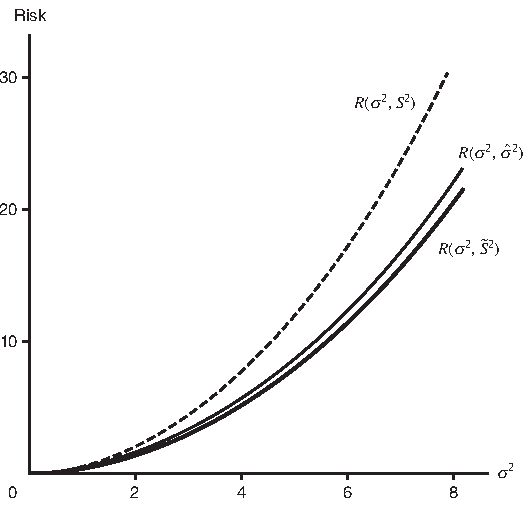
\includegraphics[width=.66\linewidth]{assets/chapter7/fig-7-3-2.pdf}
\caption{\autoref{ex:7.3.26}中三个方差估计量的风险函数}\label{fig:7.3.2}
\end{figure}
\begin{example}[Stein损失下的方差估计]\label{ex:7.3.27}\index{SI0658@似然}\index{SI0662@Stein损失}
再次考虑用形如$bS^2$的估计量估计总体方差$\sigma^2$.这次分析可以十分一般，只假设$X_1,\ldots,X_n$是来自某个具有正且有限方差$\sigma^2$的总体的随机样本.现在使用归于Stein的损失函数（\hyperref[bib:source176]{James和Stein 1961}；另见\hyperref[bib:source51]{Brown 1990a）}
$$L(\sigma^2,a)=\frac a{\sigma^2}-1-\log\frac a{\sigma^2}.$$
它比平方误差损失复杂，但有一些合理性质.注意，若$a=\sigma^2$，损失为零.此外，对于固定的$\sigma^2$，当$a\to0$或$a\to\infty$时，均有$L(\sigma^2,a)\to\infty$.即严重低估与严重高估受到同样严厉的惩罚.（在方差估计中，对平方误差损失的一项批评是，低估只受有限惩罚，高估则受无限惩罚.）若样本来自正态总体，这个损失函数也可从$\sigma^2$的似然函数导出，因此将良好的决策论性质与良好的似然性质联系起来（见\autoref{exercise:7.61}）.

对估计量$\delta_b=bS^2$，风险函数为
\begin{align*}
R(\sigma^2,\delta_b)&=E\left(\frac{bS^2}{\sigma^2}-1-\log\frac{bS^2}{\sigma^2}\right)\\
&=bE\frac{S^2}{\sigma^2}-1-E\log\frac{bS^2}{\sigma^2}\\
&=b-\log b-1-E\log\frac{S^2}{\sigma^2}.\qquad\left(E\frac{S^2}{\sigma^2}=1\right)
\end{align*}
量$E\log(S^2/\sigma^2)$可能是$\sigma^2$及其他总体参数的函数，但不是$b$的函数.因此，对所有$\sigma^2$，使$b-\log b$最小的$b$也使$R(\sigma^2,\delta_b)$最小，即$b=1$.所以，在$bS^2$形式的估计量中，对所有$\sigma^2$风险最小的是$\delta_1=S^2$.\footnote{译注：要作这里有限风险的比较，还需$S^2>0$几乎处处及相应对数期望有限；仅总体方差正且有限不足以保证这些条件.例如离散总体可能使$P(S^2=0)>0$，此时所有正$b$的Stein风险均为无穷，不能据该计算得到有意义的严格优劣比较.}
\end{example}
\sourcepageanchor{316}
也可用Bayes方法研究损失函数下的最优性，此时给定先验分布$\pi(\theta)$.在Bayes分析中，用该先验计算平均风险
$$\int_\Theta R(\theta,\delta)\pi(\theta)\,d\theta,$$
它称为Bayes风险（Bayes risk）.\index{SI0083@贝叶斯风险}\semanticindexanchor{83:316}对风险函数取平均，得到一个数，用来评估给定损失函数下估计量的性能.而且，可以尝试寻找使Bayes风险最小的估计量，称为关于先验$\pi$的Bayes规则（Bayes rule with respect to a prior $\pi$），\index{SI0085@先验分布}\semanticindexanchor{85:316}常记为$\delta^\pi$.

寻找给定先验$\pi$的Bayes决策规则看起来可能很困难，但实际过程相当机械化，正如下面的定理所指出的.（下面这种寻找Bayes规则的方法，在比此处更一般的情形中也适用，见\hyperref[bib:source54]{Brown和Purves 1973}.）

对于$\boldsymbol X\sim f(\boldsymbol x\mid\theta)$和$\theta\sim\pi$，决策规则$\delta$的Bayes风险可写为
$$\int_\Theta R(\theta,\delta)\pi(\theta)\,d\theta=\int_\Theta\left(\int_{\mathcal X}L(\theta,\delta(\boldsymbol x))f(\boldsymbol x\mid\theta)\,d\boldsymbol x\right)\pi(\theta)\,d\theta.$$
若写成$f(\boldsymbol x\mid\theta)\pi(\theta)=\pi(\theta\mid\boldsymbol x)m(\boldsymbol x)$，其中$\pi(\theta\mid\boldsymbol x)$是$\theta$的后验分布，$m(\boldsymbol x)$是$\boldsymbol X$的边缘分布，则Bayes风险可写为
\begin{equation}\label{eq:7.3.19}\index{SI0660@后验期望损失}\index{SI0820@后验期望损失（另见损失函数）}
\int_\Theta R(\theta,\delta)\pi(\theta)\,d\theta=\int_{\mathcal X}\left[\int_\Theta L(\theta,\delta(\boldsymbol x))\pi(\theta\mid\boldsymbol x)\,d\theta\right]m(\boldsymbol x)\,d\boldsymbol x.
\end{equation}
方括号内是损失函数关于后验分布的期望，称为后验期望损失（posterior expected \mbox{loss）.}它仅是$\boldsymbol x$的函数，不是$\theta$的函数.因此，对每个$\boldsymbol x$，若选行动$\delta(\boldsymbol x)$使后验期望损失最小，就使Bayes风险最小.

注意，现在有了构造Bayes规则的步骤：对于给定观测$\boldsymbol x$，Bayes规则应最小化后验期望损失.这与前面各小节的任何方法都很不一样.例如，考虑前面寻找最佳无偏估计量的方法.要用\autoref{thm:7.3.23}，首先须找到完备充分统计量$T$，然后找到一个函数$\phi(T)$，它是所求参数的无偏估计量.如果已经知道参数的某个无偏估计量，Rao--Blackwell定理（\autoref{thm:7.3.17}）可能有帮助；但如果想不出任何无偏估计量，该方法并不告诉我们怎样构造一个.

即使不能解析地最小化后验期望损失，也可以用数值方法计算积分并进行最小化.事实上，观测到$\boldsymbol X=\boldsymbol x$后，只需对这个特定的$\boldsymbol x$完成最小化.不过，在有些问题中，可以显式描述Bayes规则.
\needspace{7\baselineskip}
\begin{example}[两种Bayes规则]\label{ex:7.3.28}\index{SI0654@绝对误差}\index{SI0659@点估计}\index{SI0661@平方误差}\index{SI0683@均方误差}\index{SI0776@决策论}
考虑实参数$\theta$的点估计问题.
\begin{enumerate}[label=(\alph*)]
\item 对平方误差损失，后验期望损失为
$$\int_\Theta(\theta-a)^2\pi(\theta\mid\boldsymbol x)\,d\theta=E((\theta-a)^2\mid\boldsymbol X=\boldsymbol x).$$
这里$\theta$为分布是$\pi(\theta\mid\boldsymbol x)$的随机变量.由\autoref{ex:2.2.6}，$\delta^\pi(\boldsymbol x)=E(\theta\mid\boldsymbol x)$使该期望最小.所以Bayes规则是后验分布的均值.
\item 对绝对误差损失，后验期望损失为$E(|\theta-a|\mid\boldsymbol X=\boldsymbol x)$.应用\autoref{exercise:2.18}可知，取$\delta^\pi(\boldsymbol x)$为$\pi(\theta\mid\boldsymbol x)$的中位数，即使它最小.
\end{enumerate}
\end{example}
\sourcepageanchor{317}
\begin{table}[H]
\centering
\caption{二项分布参数$p$的三个估计量}\label{tab:7.3.1}
\begin{tabular}{rrrr}
\hline
\multicolumn{4}{c}{$n=10$，先验$\pi(p)\sim\operatorname{uniform}(0,1)$}\\
$y$&MLE&\shortstack{Bayes\\绝对误差}&\shortstack{Bayes\\平方误差}\\\hline
0&.0000&.0611&.0833\\
1&.1000&.1480&.1667\\
2&.2000&.2358&.2500\\
3&.3000&.3238&.3333\\
4&.4000&.4119&.4167\\
5&.5000&.5000&.5000\\
6&.6000&.5881&.5833\\
7&.7000&.6762&.6667\\
8&.8000&.7642&.7500\\
9&.9000&.8520&.8333\\
10&1.0000&.9389&.9137\footnotemark\\\hline
\end{tabular}
\end{table}
\footnotetext{译注：原表最后一项为$.9137$，按$(y+1)/(n+2)=11/12$计算，应为$.9167$.原数值保留.}
在\autoref{sec:7.2.3}中，所讨论的Bayes估计量为后验均值$\delta^\pi(\boldsymbol x)=E(\theta\mid\boldsymbol x)$.现在知道，它是平方误差损失下的Bayes估计量.若认为另一种损失函数比平方误差损失更合适，Bayes估计量可能是不同的统计量.
\begin{example}[正态分布的Bayes估计]\label{ex:7.3.29}
设$X_1,\ldots,X_n$是来自$n(\theta,\sigma^2)$总体的随机样本，先验$\pi(\theta)$为$n(\mu,\tau^2)$.$\sigma^2$、$\mu$和$\tau^2$都已知.在\autoref{ex:7.2.16}及其在\autoref{exercise:7.22}中的推广里，已得到给定$\bar X=\bar x$时$\theta$的后验分布为正态，且
$$E(\theta\mid\bar x)=\frac{\tau^2}{\tau^2+(\sigma^2/n)}\bar x+\frac{\sigma^2/n}{\tau^2+(\sigma^2/n)}\mu,$$
以及
$$\operatorname{Var}(\theta\mid\bar x)=\frac{\tau^2\sigma^2/n}{\tau^2+(\sigma^2/n)}.$$
在平方误差损失下，Bayes估计量为$\delta^\pi(\boldsymbol x)=E(\theta\mid\bar x)$.由于后验分布为正态，它关于均值对称，$\pi(\theta\mid\boldsymbol x)$的中位数等于$E(\theta\mid\boldsymbol x)$.因此，在绝对误差损失下，Bayes估计量也为$\delta^\pi(\boldsymbol x)=E(\theta\mid\bar x)$.
\end{example}
\begin{example}[二项分布的Bayes估计]\label{ex:7.3.30}\index{SI0777@二项}
设$X_1,\ldots,X_n$独立同分布于$\operatorname{Bernoulli}(p)$，令$Y=\sum X_i$.假设$p$的先验为$\operatorname{beta}(\alpha,\beta)$.在\autoref{ex:7.2.14}中，已发现后验分布只通过$Y=y$的观测值依赖样本，且为$\operatorname{beta}(y+\alpha,n-y+\beta)$.因此，$\delta^\pi(y)=E(p\mid y)=(y+\alpha)/(\alpha+\beta+n)$是平方误差损失下$p$的Bayes估计量.

对于绝对误差损失，需要寻找$\pi(p\mid y)=\operatorname{beta}(y+\alpha,n-y+\beta)$的中位数.一般没有简单表达式.中位数隐式定义为满足
$$\int_0^m\frac{\Gamma(\alpha+\beta+n)}{\Gamma(y+\alpha)\Gamma(n-y+\beta)}p^{y+\alpha-1}(1-p)^{n-y+\beta-1}\,dp=\frac12$$
的数$m$.可以数值计算该积分，近似找出满足等式的$m$.对于$n=10$、$\alpha=\beta=1$，即$\operatorname{uniform}(0,1)$先验，我们已作了这种计算.绝对误差损失的Bayes估计量列于\autoref{tab:7.3.1}；表中还列出前面导出的平方误差损失的Bayes估计量，以及MLE $\widehat p=y/n$.

注意\autoref{tab:7.3.1}：与MLE不同，即使$y=0$或$n$，两个Bayes估计量都不会把$p$估为0或1.Bayes估计量通常不会取参数空间中的
\sourcepageanchor{318}
极端值.不论样本量多大，先验始终对估计量有一定影响，倾向于把它从极端值拉开.从上面$E(p\mid y)$的表达式可见，即使$y=0$且$n$很大，Bayes估计量仍是正数.
\end{example}
